\documentclass[11pt]{article}
\usepackage[margin=1in, top=1in]{geometry}
\usepackage[all]{nowidow}
\usepackage[hyperfigures=true, hidelinks, pdfhighlight=/N]{hyperref}
\usepackage[separate-uncertainty=true, group-digits=true]{siunitx}
\usepackage{graphicx,amsmath,physics,tabto,float,amssymb,pgfplots,verbatim,tcolorbox}
\usepackage{listings,xcolor,subfig,caption,import,wrapfig,enumitem}
\usepackage[version=4]{mhchem}
\usepackage[noabbrev]{cleveref}
\newcommand{\creflastconjunction}{, and\nobreakspace}
\newcommand{\mb}[1]{\mathbf{#1}}
\definecolor{stringcolor}{HTML}{C792EA}
\definecolor{codeblue}{HTML}{2162DB}
\definecolor{commentcolor}{HTML}{4A6E46}
\captionsetup{font=small, belowskip=0pt}
\lstdefinestyle{appendix}{
    basicstyle=\ttfamily\footnotesize,commentstyle=\color{commentcolor},keywordstyle=\color{codeblue},
    stringstyle=\color{stringcolor},showstringspaces=false,numbers=left,upquote=true,captionpos=t,
    abovecaptionskip=12pt,belowcaptionskip=12pt,language=Python,breaklines=true,frame=single}
\lstdefinestyle{inline}{
    basicstyle=\ttfamily\footnotesize,commentstyle=\color{commentcolor},keywordstyle=\color{codeblue},
    stringstyle=\color{stringcolor},showstringspaces=false,numbers=left,upquote=true,frame=tb,
    captionpos=b,language=Python}
\renewcommand{\lstlistingname}{Appendix}
\pgfplotsset{compat=1.17}

\begin{document}

\begin{center}
    \textbf{CP Tut 4}\hspace{1.5in}\textbf{KDSMIL001}\hspace{1.5in}\textbf{04-06-2022}
\end{center}
\rule{\textwidth}{1pt}

\begin{enumerate}
    \item \begin{enumerate}
        \item We aim to approximate the advection-diffusion equation:
        \begin{equation}
            \epsilon\frac{d^2u}{dx^2}-\frac{du}{dx}=0
            \label{eqn:advection-diffusion}
        \end{equation}
        where $u(0)=2$ and $u(1)=1$ with $\epsilon$ simply a constant. We can begin by approximating the derivatives with central difference methods. Using a grid spacing of $\Delta x$ and using notation $u(x_i)=u_i$:
        \begin{equation*}
            \epsilon\frac{u_{i-1}-2u_i+u_{i+1}}{\Delta x^2}-\frac{u_{i+1}-u_{i-1}}{2\Delta x}=0
        \end{equation*}
        Rearranging this to find coefficients of $u_i$'s we have
        \begin{equation*}
            u_{i-1}\underbrace{\left(\epsilon+\frac{\Delta x}{2}\right)}_\alpha +u_i\underbrace{(-2\epsilon)}_\gamma +u_{i+1}\underbrace{\left(\epsilon-\frac{\Delta x}{2}\right)}_\beta=0.
        \end{equation*}
        From this, we construct our matrix equation. Note we are using $N+2$ points, starting from $x_0$
        \begin{equation*}
            \begin{pmatrix}
                \gamma & \beta & 0 & \cdots & 0 \\
                \alpha & \gamma & \beta & \cdots & 0 \\
                0 & \ddots & \ddots & \ddots & \vdots \\
                \vdots & \cdots & \alpha & \gamma & \beta \\
                0 & \cdots & \cdots & \alpha & \gamma
            \end{pmatrix}
            \begin{pmatrix}
                u_1 \\
                u_2 \\
                \vdots \\
                u_{N-1} \\
                u_N
            \end{pmatrix}
            =
            \begin{pmatrix}
                -\alpha u_0 \\
                0 \\
                \vdots \\
                0 \\
                -\beta u_{N+1}
            \end{pmatrix}
        \end{equation*}
        Since we know $u_0$ and $u_{N+1}$ from the BCs, we have an implicit system to solve here, which we can solve with any linear algebra package.

        \item We now implement this method for $\epsilon=0.1$ in the \texttt{q1b} method submitted. Important to note are the additions of the BCs to the ends of the solution. The solution is shown in \cref{fig:q1b}. 
        
        \begin{figure}[h]
            \begin{center}
                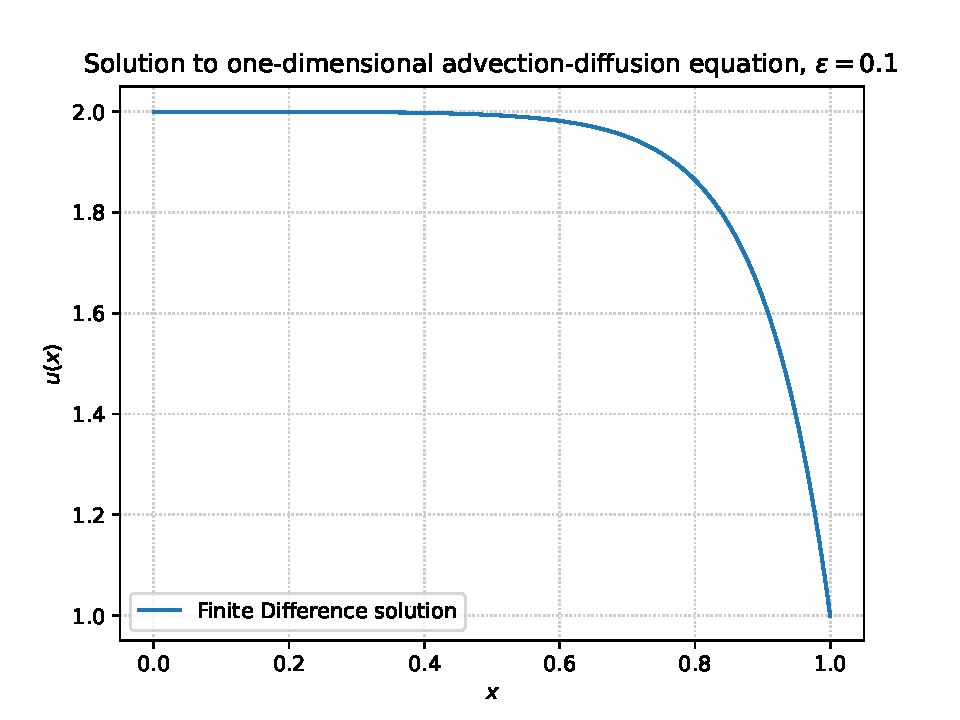
\includegraphics[width=.6\textwidth]{Plots/q1b.pdf}
                \caption{Finite difference solution to the advection-diffusion equation shown in \cref{eqn:advection-diffusion} with $\epsilon=0.1$. Central differences were used to approximate the derivatives on a grid of 1000 points.}
                \label{fig:q1b}
            \end{center}
        \end{figure}
        
        \item Now when setting $\epsilon=0.0001$, we see instability as $x\rightarrow1$, so we implement the upwinding technique, which simply involves changing the first derivative from central difference to backward difference. This gives
        \begin{align*}
            0&=\epsilon\frac{u_{i-1}-2u_i+u_{i+1}}{\Delta x^2}-\frac{u_{i}-u_{i-1}}{\Delta x}\\
            \implies0&=u_{i-1}\underbrace{\left(\epsilon+\Delta x\right)}_\alpha +u_i\underbrace{(-2\epsilon-\Delta x)}_\gamma +u_{i+1}\underbrace{\left(\epsilon\right)}_\beta.
        \end{align*}
        The matrix equation looks identical to before, and it leads to \cref{fig:q1c}.

        \begin{figure}[h]
            \begin{center}
                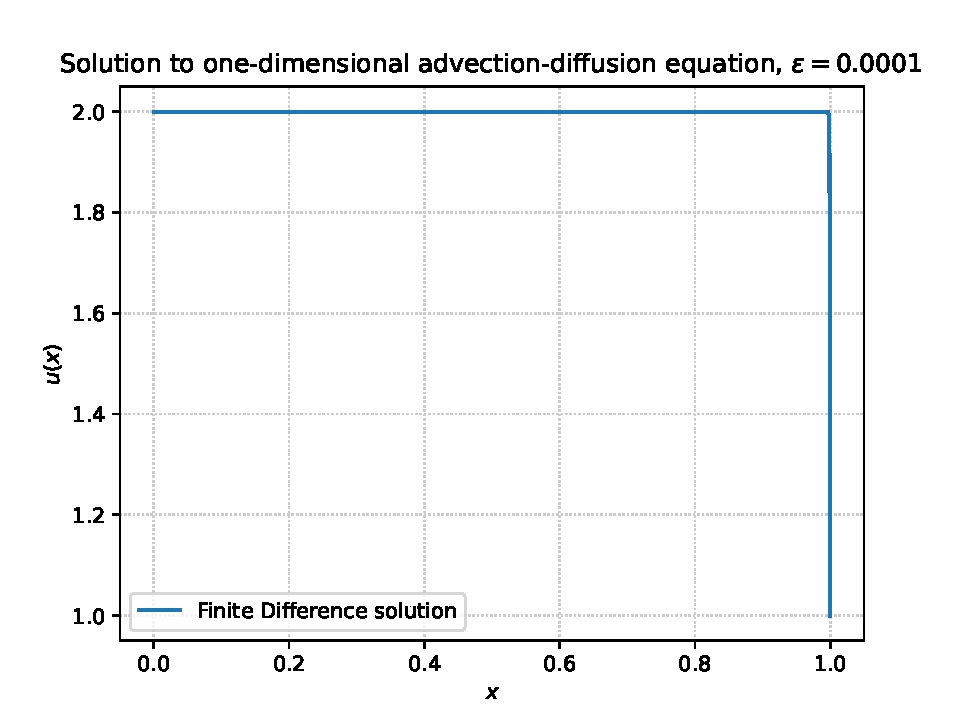
\includegraphics[width=.6\textwidth]{Plots/q1c.pdf}
                \caption{Finite difference solution to the advection-diffusion equation shown in \cref{eqn:advection-diffusion} with $\epsilon=0.0001$. A central difference was used for the second derivative, while upwinding was implemented for the first derivative, so a backwards difference was used. 1000 grid points were used.}
                \label{fig:q1c}
            \end{center}
        \end{figure}

        \item Now we want to create an explicit scheme by including a time dependence:
        \begin{equation}
            \epsilon\frac{d^2u}{dx^2}-\frac{du}{dx}=\frac{du}{dt}
            \label{eqn:time-dep}
        \end{equation}
        Once again we approximate the spatial derivatives with central differences, and then the time derivative with a forward difference. We use the notation $u(x_i, t_j)=u_{ij}$ and use a grid spacing for time of $\Delta t$:
        \begin{equation*}
            \epsilon\frac{u_{i-1,j}-2u_{i,j}+u_{i+1,j}}{\Delta x^2}-\frac{u_{i+1,j}-u_{i-1,j}}{2\Delta x}=\frac{u_{i,j+1}-u_{i,j}}{\Delta t}
        \end{equation*}
        Now we can rearrange as before, solving for the value of $u$ at the next time step:
        \begin{equation*}
            u_{i,j+1}=u_{i-1,j}\underbrace{\left(\frac{\epsilon}{\Delta x^2}+\frac{1}{2\Delta x}\right)\Delta t}_\alpha + u_{i,j}\underbrace{\left(\frac{-2\epsilon}{\Delta x^2}+\frac{1}{\Delta t}\right)\Delta t}_\gamma + u_{i+1,j}\underbrace{\left(\frac{\epsilon}{\Delta x^2}-\frac{1}{2\Delta x}\right)\Delta t}_\beta
        \end{equation*}
        The matrix equation is similar to before, but with some subtle differences:
        \begin{equation*}
            \begin{pmatrix}
                \gamma & \beta & 0 & \cdots & 0 \\
                \alpha & \gamma & \beta & \cdots & 0 \\
                0 & \ddots & \ddots & \ddots & \vdots \\
                \vdots & \cdots & \alpha & \gamma & \beta \\
                0 & \cdots & \cdots & \alpha & \gamma
            \end{pmatrix}
            \begin{pmatrix}
                u_{1,j} \\
                u_{2,j} \\
                \vdots \\
                u_{N-1,j} \\
                u_{N,j}
            \end{pmatrix}
            =
            \begin{pmatrix}
                u_{1,j+1}-\alpha u_{0,j} \\
                u_{2,j+1} \\
                \vdots \\
                u_{N-1,j+1} \\
                u_{N,j+1}-\beta u_{N+1,j}
            \end{pmatrix}
        \end{equation*}
        What's important to note here is that this equation doesn't need to be inverted as we want what's on the RHS. All that needs to be done, after multiplying the current guess by the matrix, is to add on the $\alpha u_{0,j}$ and $\beta u_{N+1,j}$ to the first and last elements respectively, and then tack on the boundary conditions to either end. \\
        We do this until a condition is met, which we choose to be that the total change in the solution from one time step to the next to be less than 1. This is fairly arbitrary but it gave a reasonable result without taking too long. \Cref{fig:q1d} shows the outcome of this method. \\
        One quirk of this method is that care needs to be taken to avoid instability. With $\Delta x=0.01$ we needed to use $\Delta t=0.00001$ or else weird things would happen. There is an analytic expression for the relationship between $\Delta x$ and $\Delta t$ but I'm not sure what it is. We can see in the plot that it took around \num[]{150000} time steps to reach a reasonable solution, and that number will go up dramatically if more accuracy is required, so this method is not particularly computationally efficient, but it works.

        \begin{figure}[H]
            \begin{center}
                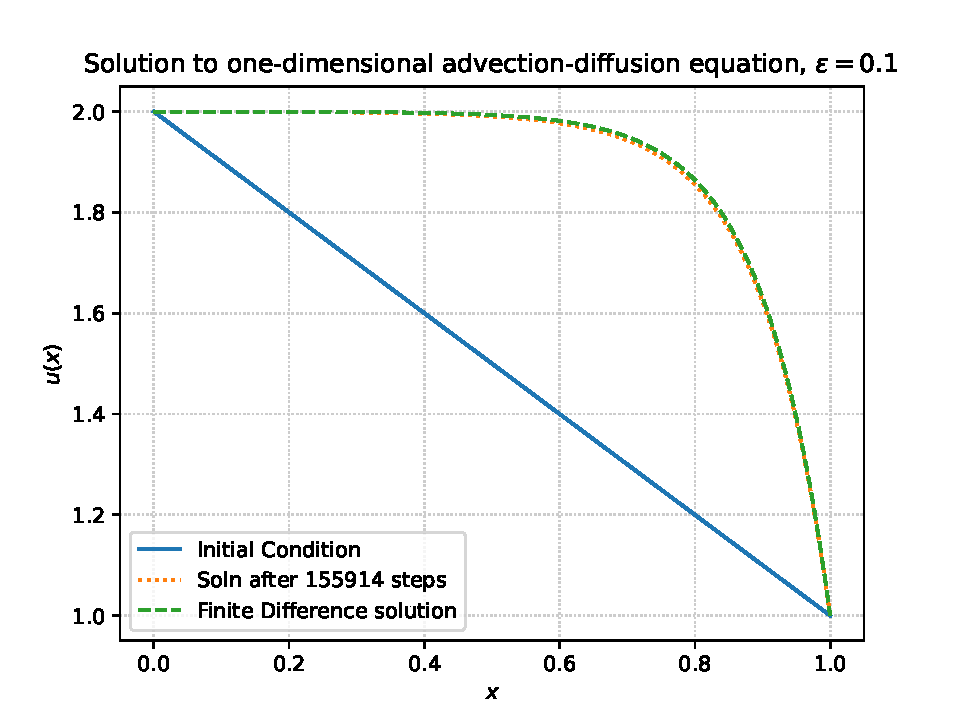
\includegraphics[width=.6\textwidth]{Plots/q1d.pdf}
                \caption{Solution to the advection-diffusion equation found by extending it to a PDE, known as the convection-diffusion equation, and solving that explicitly with a finite difference scheme. The PDE solution is shown alongside the initial condition ($u=-x+2$) used as well as the solution found in part b. $\epsilon=0.1$.}
                \label{fig:q1d}
            \end{center}
        \end{figure}
    \end{enumerate}

    \item We used a method based on the Metropolis method to simulate the Ising model, where at each step a random particle in the grid is flipped and its energy change $\Delta E$ calculated. If that energy change is less than or equal to 0, the configuration is accepted and the loop runs again, and if not then it's accepted with the Boltzmann probability $p=\exp(-\Delta E/k_B T)$ for that energy change. For ease of plotting and interpretation we have set $k_B=1$. \\
    That loop is run until each particle has statistically had the chance to flip (~\num[]{1000} in our case), and then a magnetisation calculated by finding the average of all the spins $s_i$ of the $N$ particles:
    \begin{equation*}
        M=\frac{\sum_i s_i}{N}
    \end{equation*}
    In theory, this should be done a number of times for each temperature and the average of those magnetisations is then the representative magnetisation for that temperature. To shortcut this, we let the simulation run for \num[]{10000} flips and then averaged the magnetisation from the last \num[]{7000} flips, skipping \num[]{500} each time so as not to have any correlation. We disregard the first \num[]{3000} magnetisations to be safe, as the system is still reaching an equilibrium at that point.\\
    \Cref{fig:q2} shows the results of this simulation. We can clearly see the phase change at $T\approx2.3$, as expected. 
    
    \begin{figure}[h]
        \begin{center}
            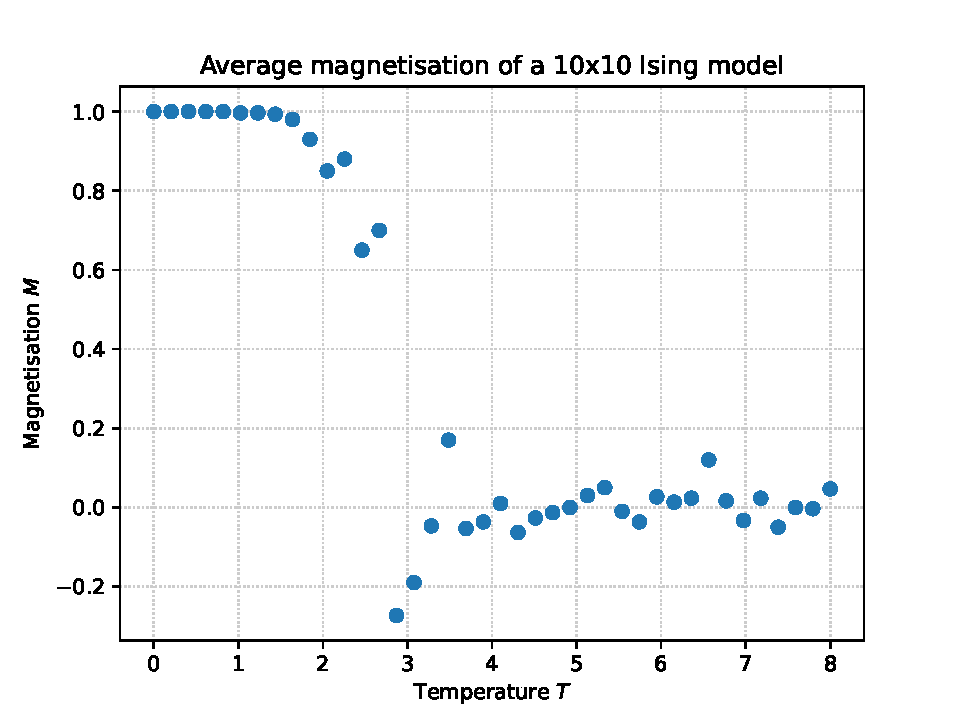
\includegraphics[width=.6\textwidth]{Plots/q2.pdf}
            \caption{Magnetisation as a function of temperature for a $10\times10$ Ising model. Note that $k_B=1$ so $T$ is in units of $K/k_B$ and $M$ is fractional magnetisation, relative to full magnetisation. For each run, the initial grid was set to all be spin-up, to make the plotting a bit nicer.}
            \label{fig:q2}
        \end{center}
    \end{figure}

    


\end{enumerate}

\end{document}